\documentclass[12pt,a4paper,dvipdfmx]{jsarticle}
\usepackage[dvipdfmx]{graphicx}
\usepackage[margin=30truemm]{geometry}
\usepackage[utf8]{inputenc}
\usepackage[T1]{fontenc}
\usepackage{pgfplots}


\begin{document}

\begin{figure}[htbp]
    \centering
    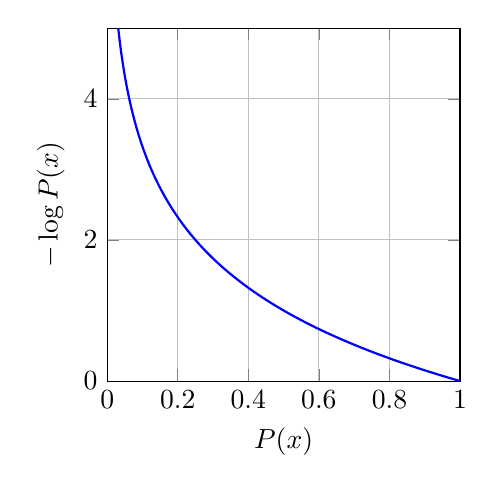
\begin{tikzpicture}
        \begin{axis}[
            domain=0.01:1,
            samples=200,
            xlabel={\( P(x) \)},
            ylabel={\( -\log P(x) \)},
            ymin=0, ymax=5,
            xmin=0, xmax=1,
            grid=major,
            width=0.5\textwidth,
            height=0.5\textwidth,
        ]
            \addplot[thick, blue] {-log2(x)};
        \end{axis}
    \end{tikzpicture}
    \caption{Self-information as a function of probability \( P(x) \).}
    \label{fig:self_info}
\end{figure}

\end{document}